
\chapter{Imagens}

A utilização de imagens em trabalhos acadêmicos é muito comum, de modo que a manipulação de imagens merece uma atenção especial. Todos os mecanismo do \LaTeX\ para a manipulação de imagens podem ser utilizados com a classe estilo, mas algumas tarefas mais rotineiras podem ter sua execução otimizada.

A classe estilo pode ser utilizada com qualquer tipo de imagem, mas a configuração padrão aceita os formatos mais comuns, a saber: .jpg, .png e .pdf. Adotar desses formatos como padrão justifica-se por que eles são extremamente comuns. O conteúdo desse capítulo presume que o arquivo da imagem esteja em um desses formatos.


\section{Inclusão de imagem}


Imagem é diferente dos outros elementos que compõem um texto, não pode ser dividida em nenhuma circunstância e devem vir acompanhadas de uma legenda
e/ou referência.

Imagens são inseridas com \verb|\includegraphics}{arquivo}|, são 
aceitas imagens nos formatos .jpg, .png, .pdf quando o objetivo for gerar pdf 
direto do tex, para gerar dvi a imagem deve estar no formato .ps ou .eps.

\begin{tcolorbox}
\begin{lstlisting}
    
\includegraphics{Logo} %%% insere a imagem
\end{lstlisting}
\end{tcolorbox}

\includegraphics{Logo}

A classe estilo procura as imagens primeiro em uma pasta chamada "\textsf{Imagens}"\, que deve estar no mesmo diretório de seu arquivo tex, se essa pasta não existir a imagem será procurada na mesma pasta do arquivo tex, se o arquivo não existir a compilação falhará e será exibida a mensagem de erro: \textit{File not found}.

O comando \verb|includegraphics{arquivo}| apenas insere a imagem, para que tenha legenda é necessário colocá-la dentro de um ambiente \verb|figure|, onde também é possível controlar seu posicionamento horizontal.
\begin{tcolorbox}
\begin{lstlisting}
\begin{figure}[H]
    \centering %%% Centraliza a imagem
    
\includegraphics{Logo} %%% Insere a imagem
    \caption{Este é o logotipo da UFRRJ} %%% Legenda da imagem
    \label{Logorural} %%% Marca para fazer referência cruzada
\end{figure}
\end{lstlisting}
\end{tcolorbox}
\begin{figure}[H]
	\centering %%% centraliza a imagem
	
\includegraphics{Logo}
	\caption{Este é o logotipo da UFRRJ} %%% legenda da imagem
	\label{Logorural} %%% Marca para fazer referência cruzada
\end{figure}


\begin{tcolorbox}
\begin{lstlisting}
\begin{figure}[H]
   \centering
   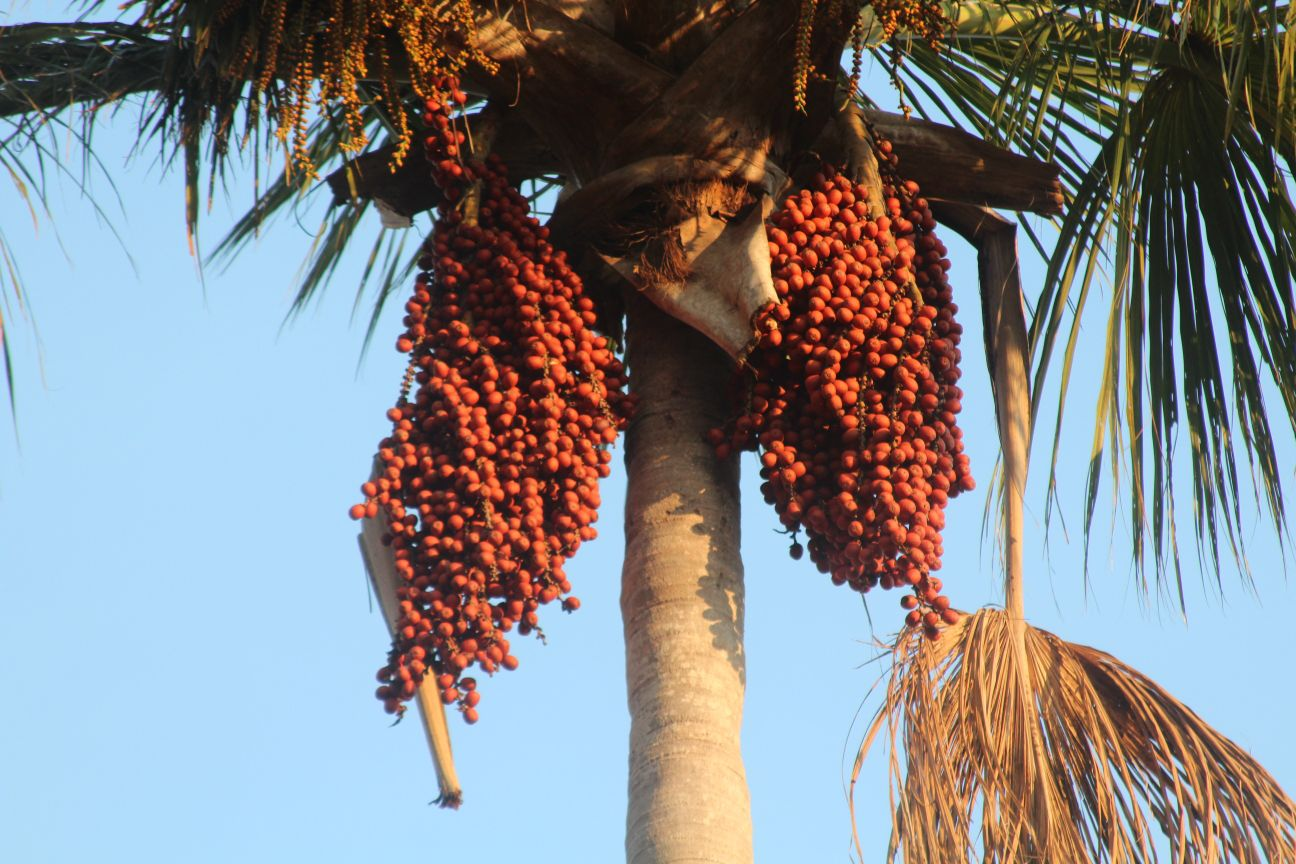
\includegraphics[scale=0.15]{Buriti}
   \caption{Imagem reduzia a $15\%$ do seu tamanho}
\end{figure}
\end{lstlisting}
\end{tcolorbox}
\begin{figure}[H]
   \centering
   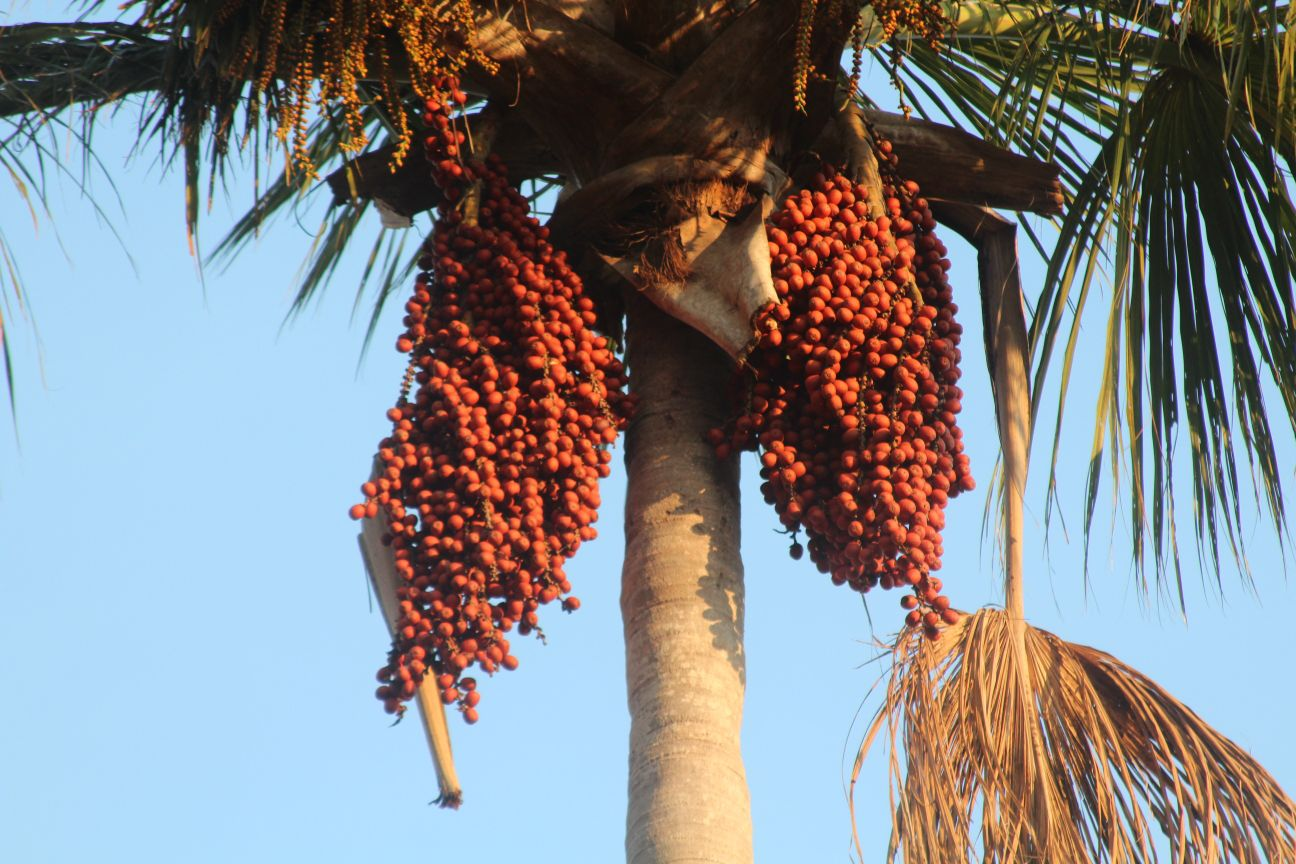
\includegraphics[scale=0.15]{Buriti}
   \caption{Imagem reduzia a $15\%$ do seu tamanho}
   \label{primeira}
\end{figure}

Uma opção muito comum ao lidar com imagem consiste em ajustar seu tamanho para coincidir com a largura da página, o comando \verb|\resizebox| faz esse ajuste
\begin{tcolorbox}
\begin{lstlisting}
\begin{figure}[H]
   \resizebox{\textwidth}{!}{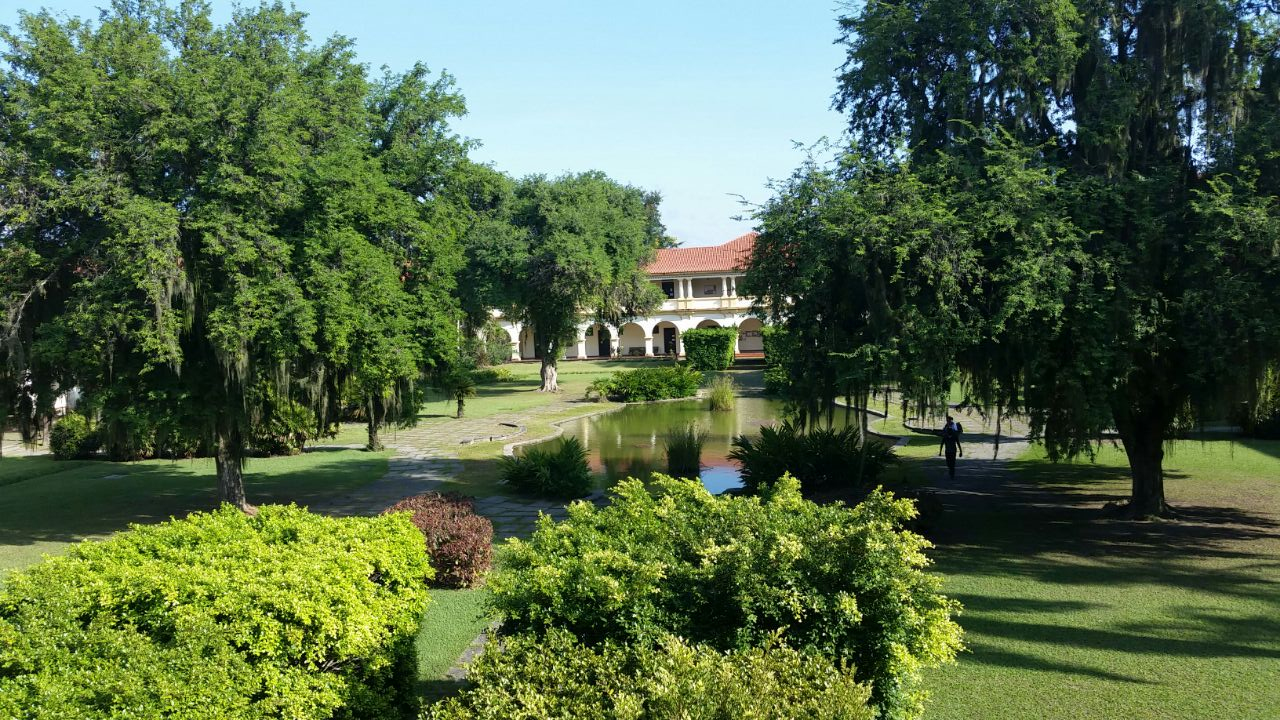
\includegraphics{RuralP1}}
   \caption{O prédio principal da UFRRJ, vulgo P1}
   \label{op1} %%% Marca para referência cruzada
\end{figure}
\end{lstlisting}
\end{tcolorbox}
\begin{figure}[H]
	\resizebox{\textwidth}{!}{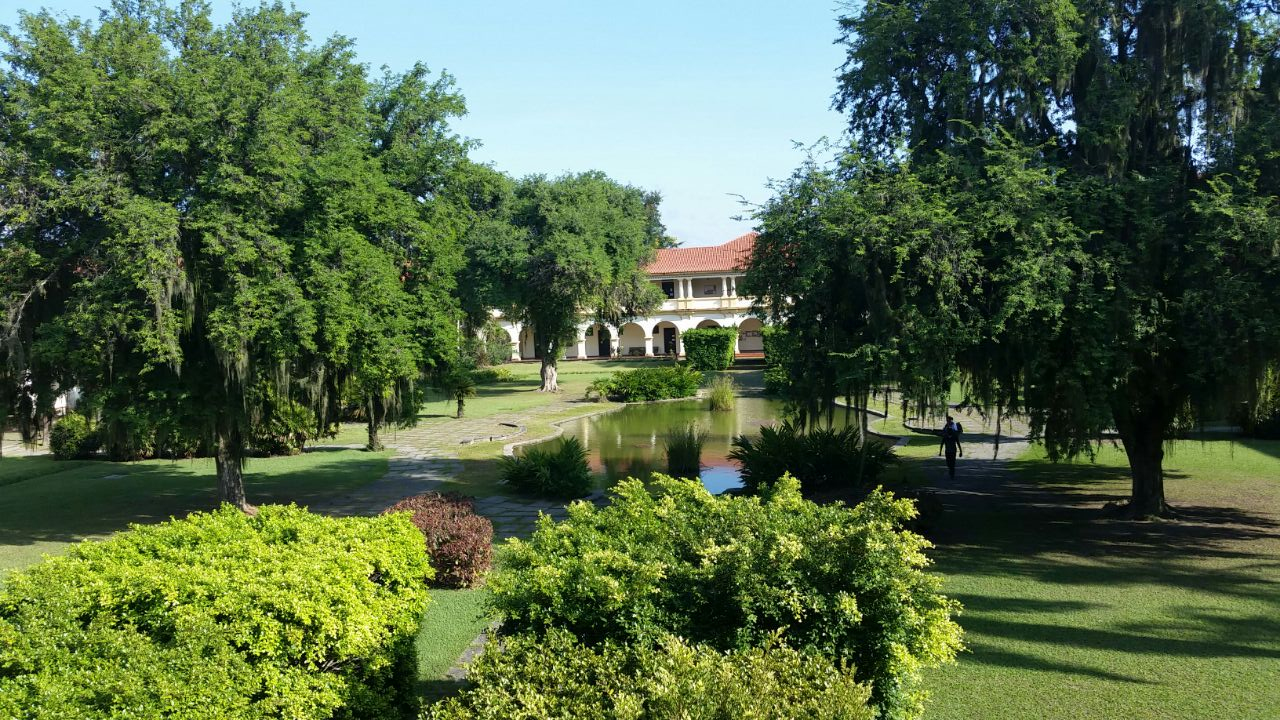
\includegraphics{RuralP1}}
	\caption{O prédio principal da UFRRJ, vulgo P1}
	\label{op1}
\end{figure}

\subsection{Girando de imagem}

É muito simples girar uma imagem no sentido horário ou anti-horário.
\begin{tcolorbox}
\begin{lstlisting}
\begin{figure}[H]
   \centering
   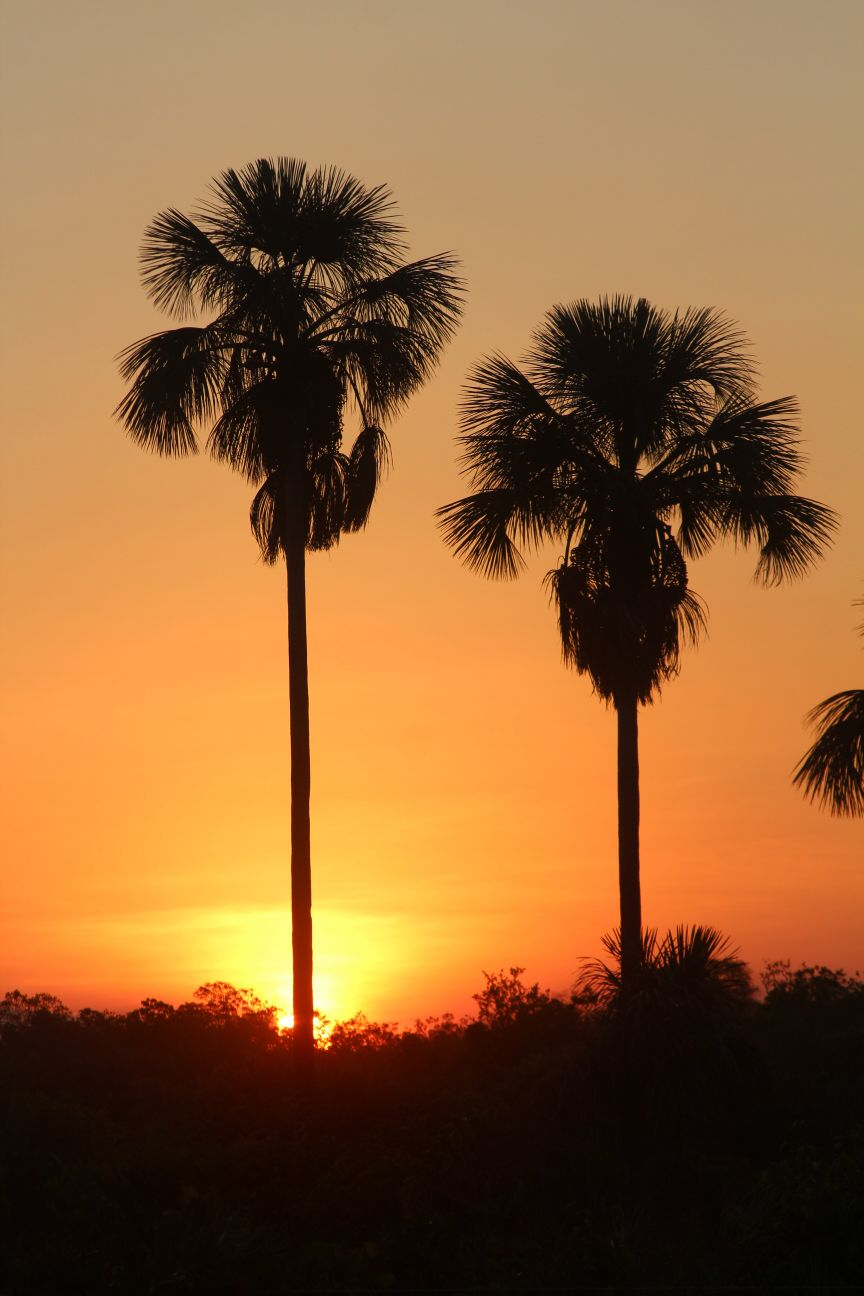
\includegraphics[scale=0.1,angle=-15]{Buritis}
   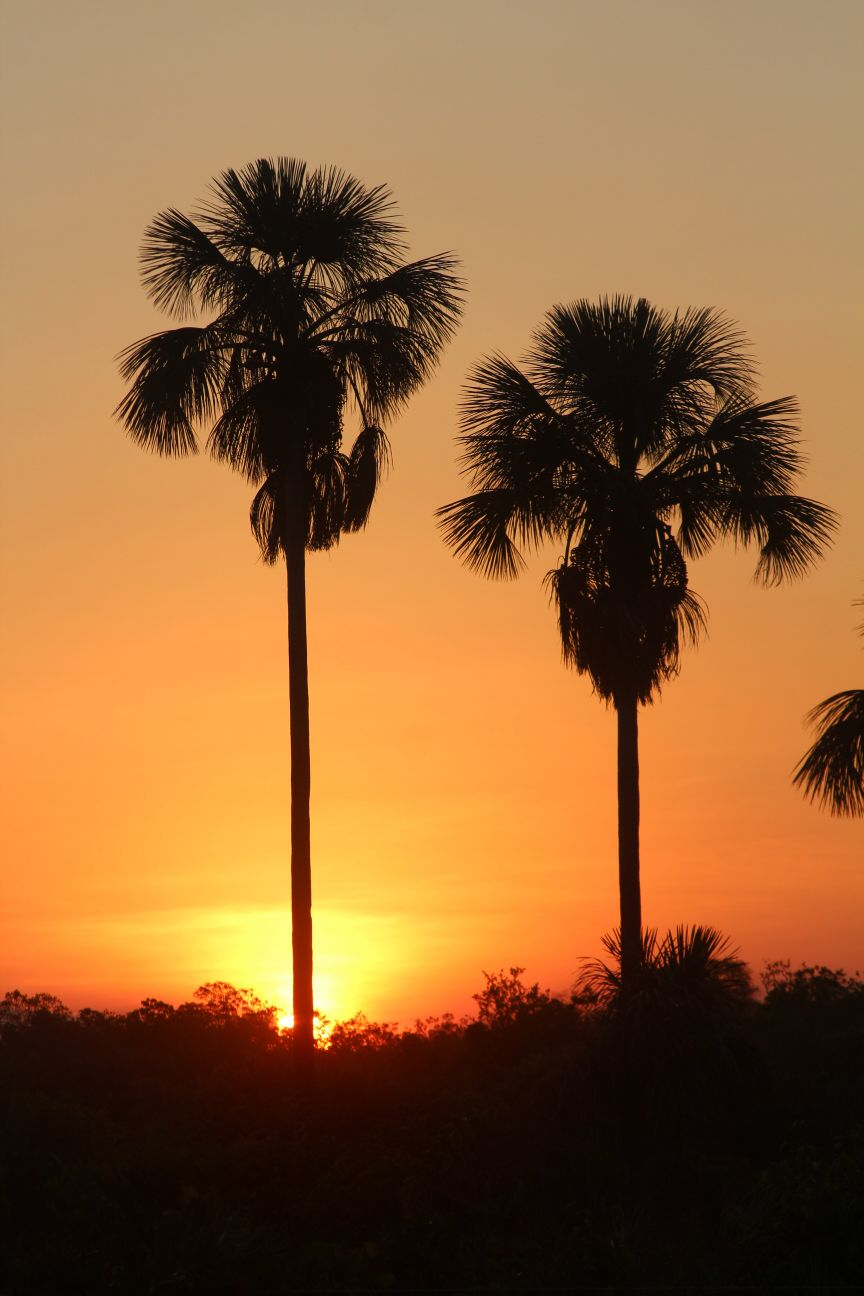
\includegraphics[scale=0.1]{Buritis}
   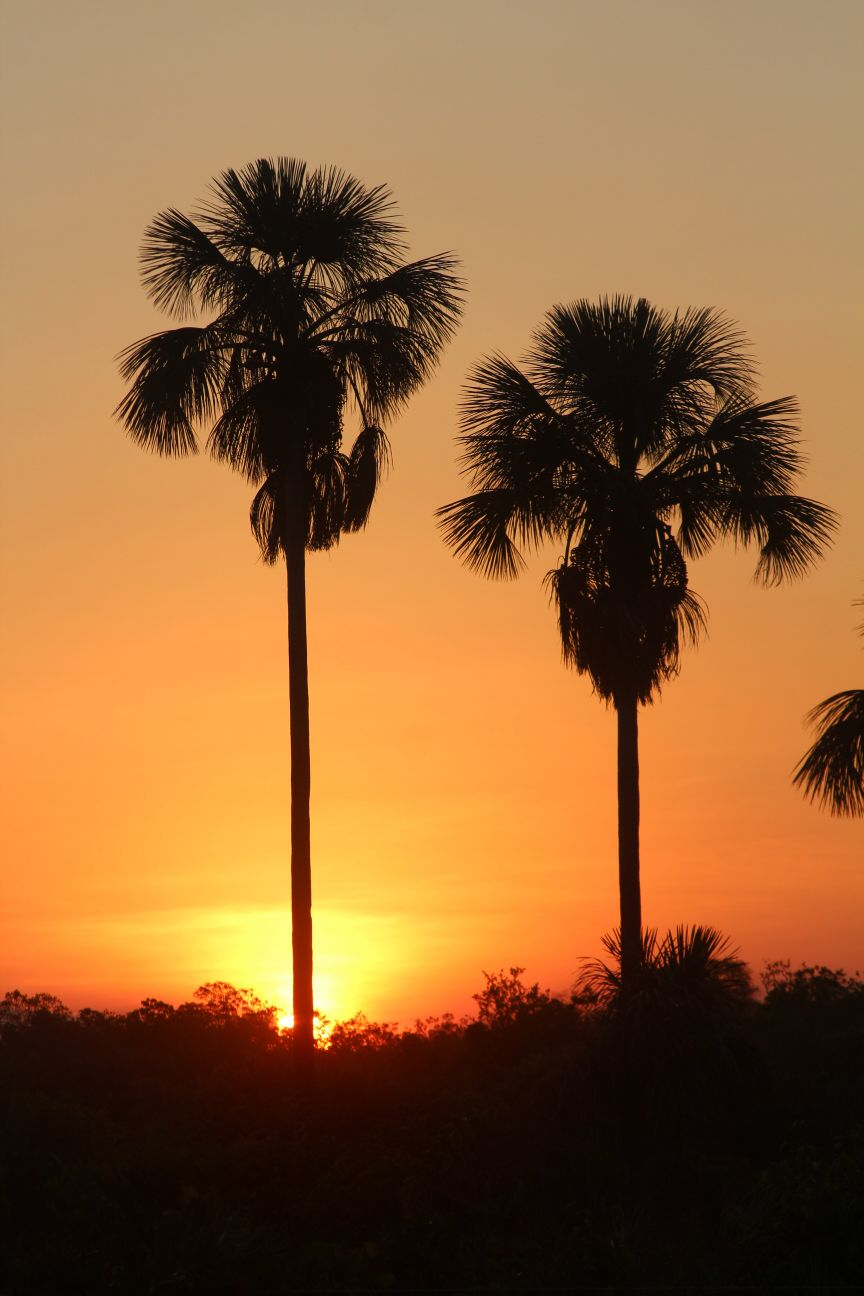
\includegraphics[scale=0.1,angle=15]{Buritis}
   \caption{Girando imagens}\label{giraas}
\end{figure}
\end{lstlisting}
\end{tcolorbox}

\begin{figure}[H]
	\centering
	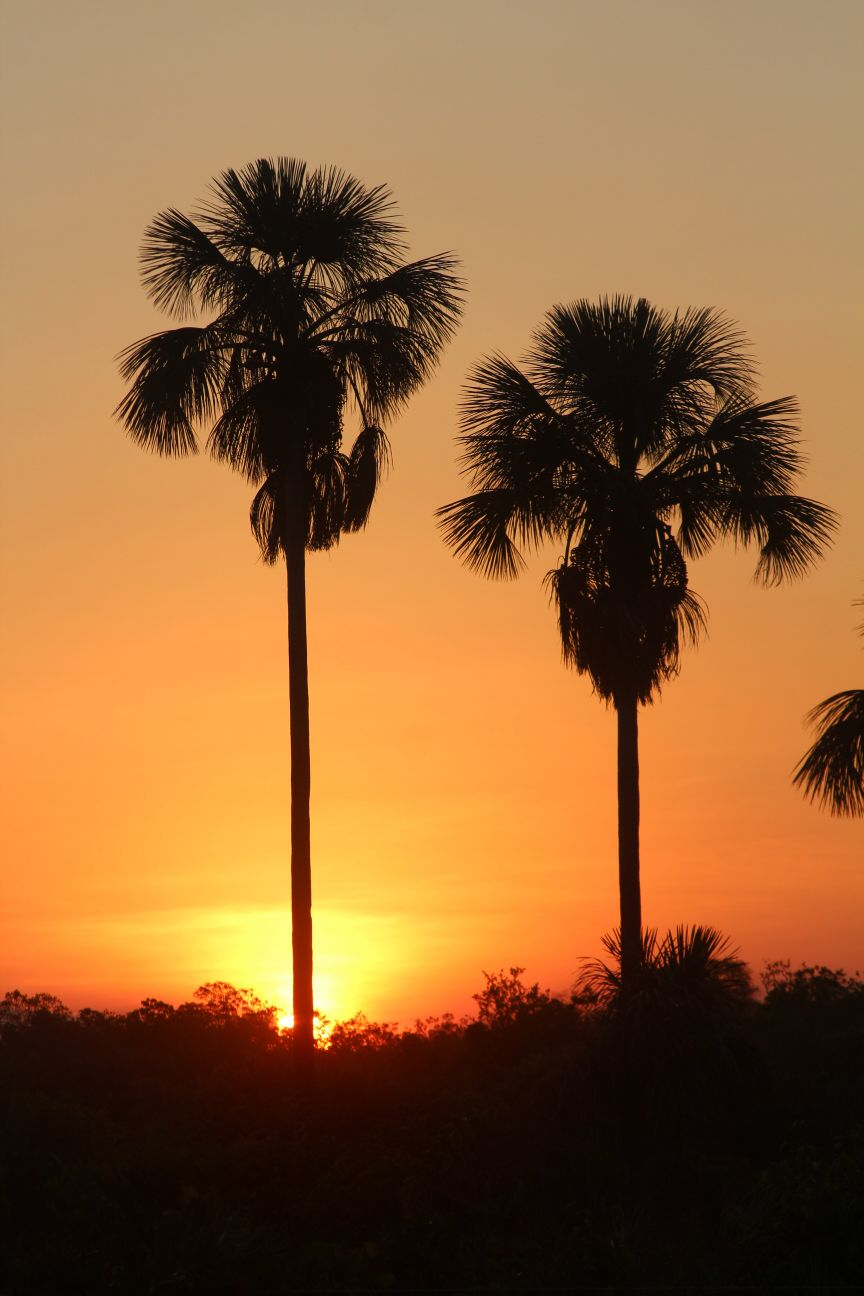
\includegraphics[scale=0.1,angle=-15]{Buritis}
	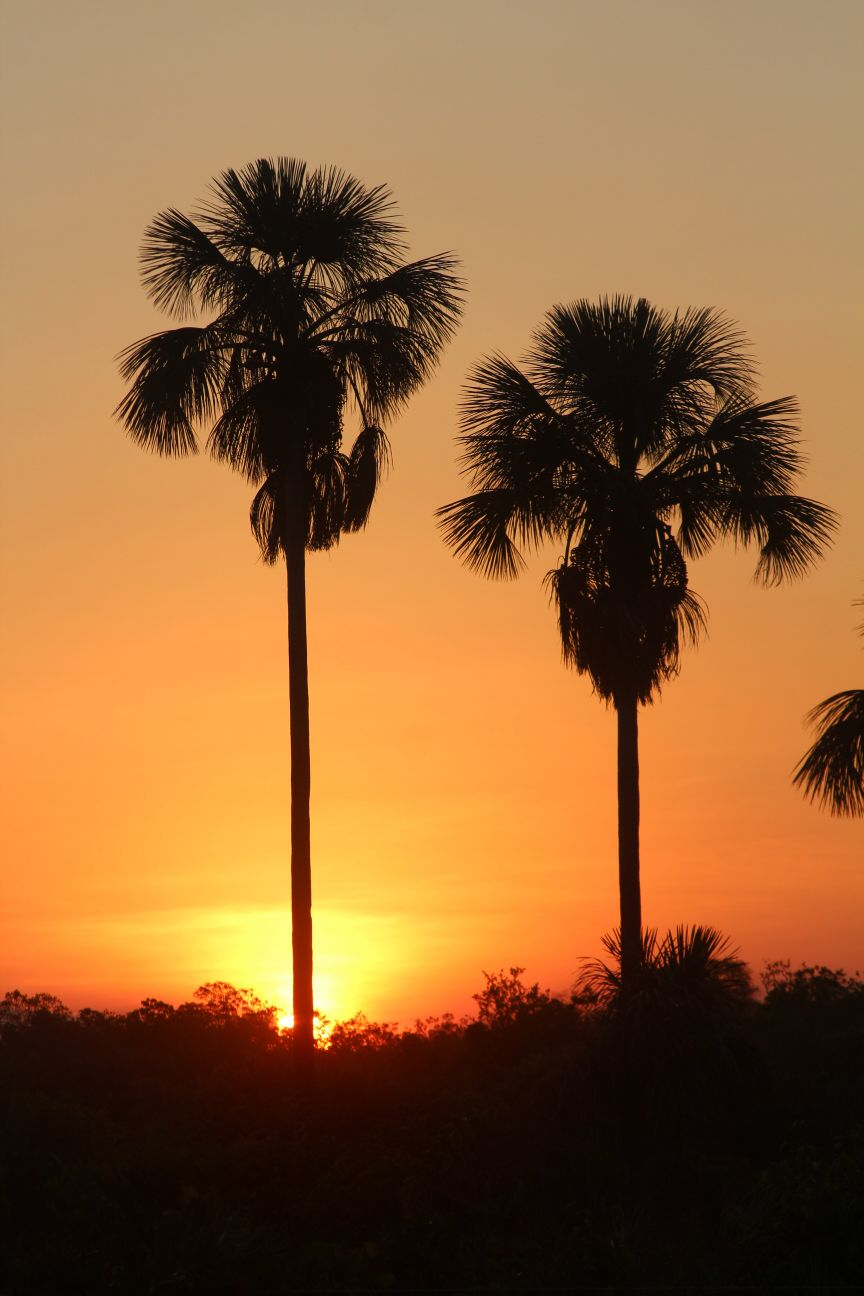
\includegraphics[scale=0.1]{Buritis}
	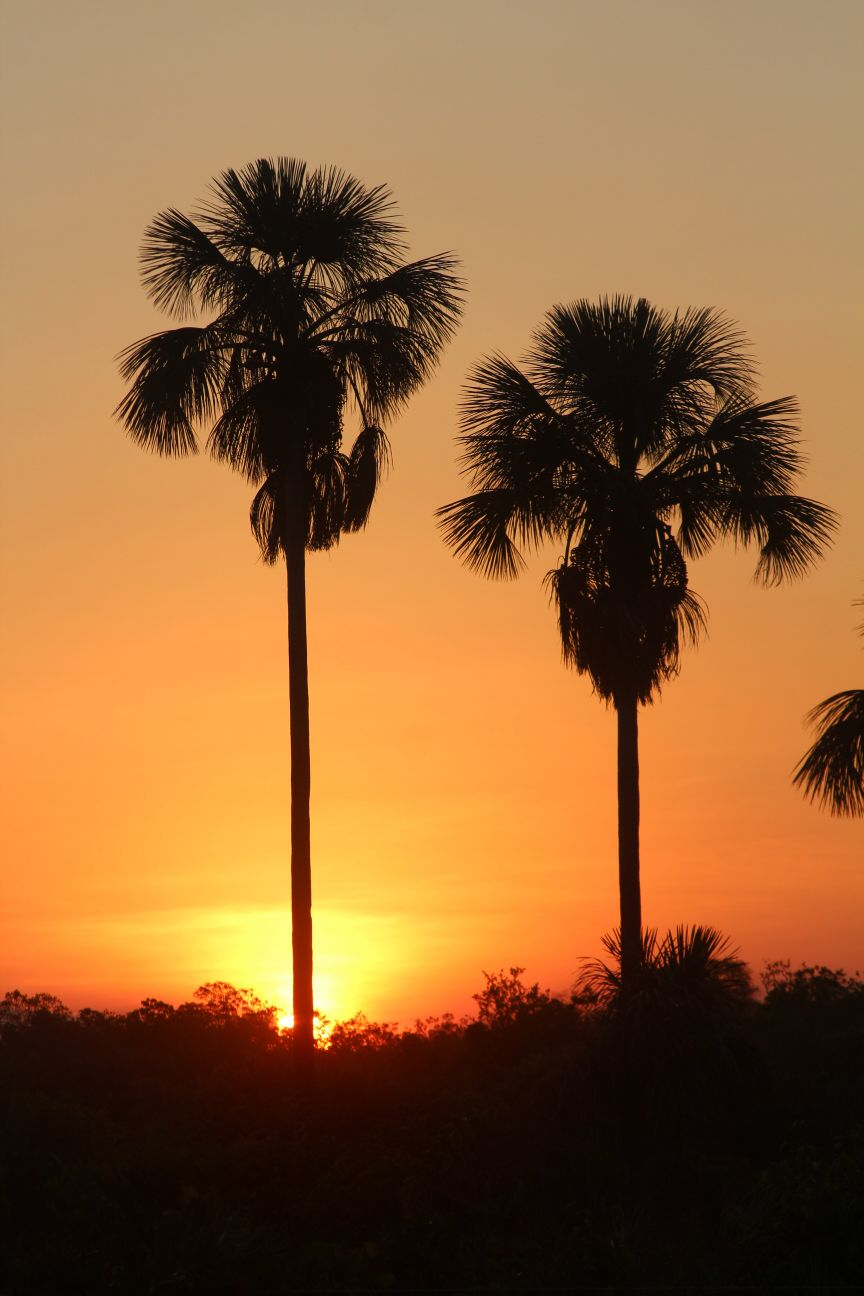
\includegraphics[scale=0.1,angle=15]{Buritis}
	\caption{Girando imagens}\label{giraas}
\end{figure}


\subsection{Imagens lado a lado}

\begin{tcolorbox}
\begin{lstlisting}
\begin{figure}[H]
   \centering
   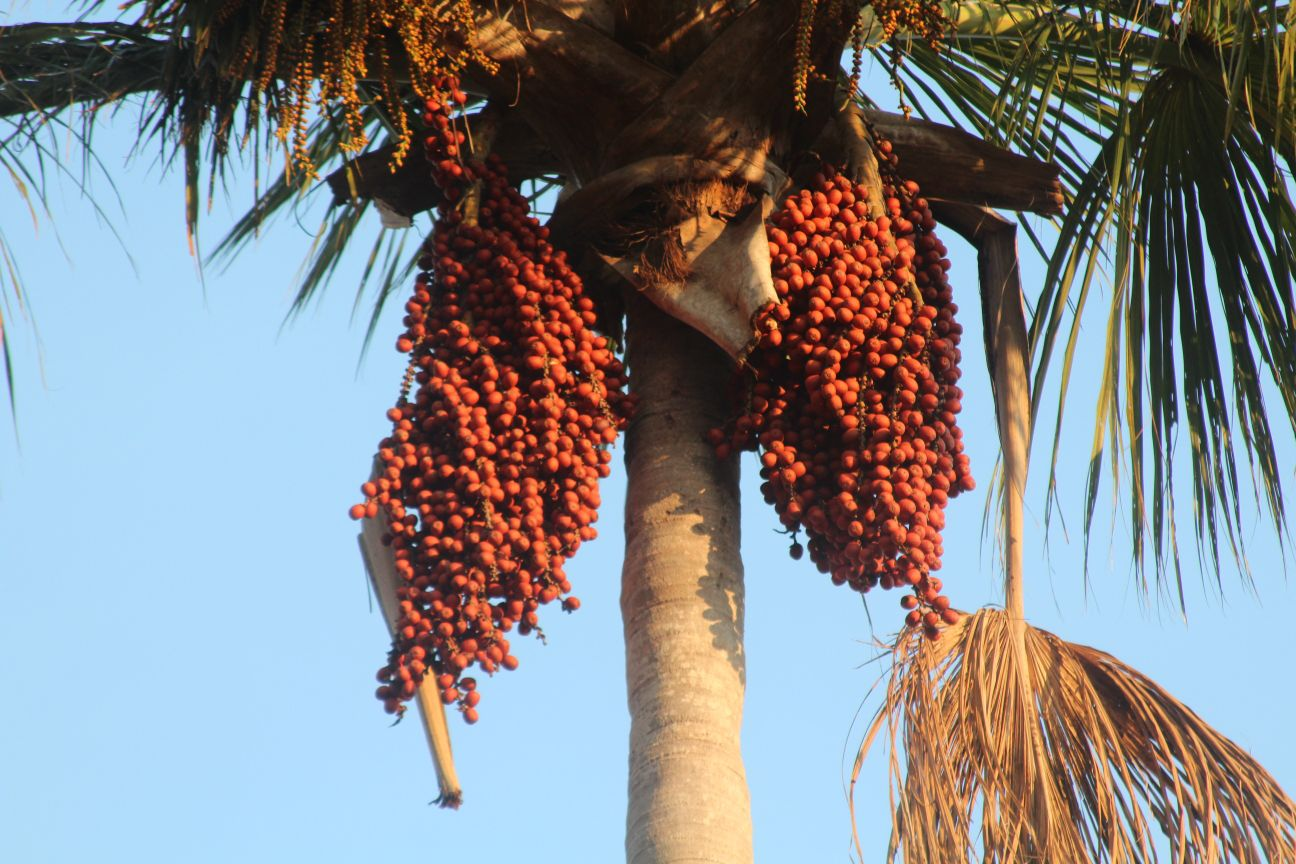
\includegraphics[scale=0.1]{Buriti}
   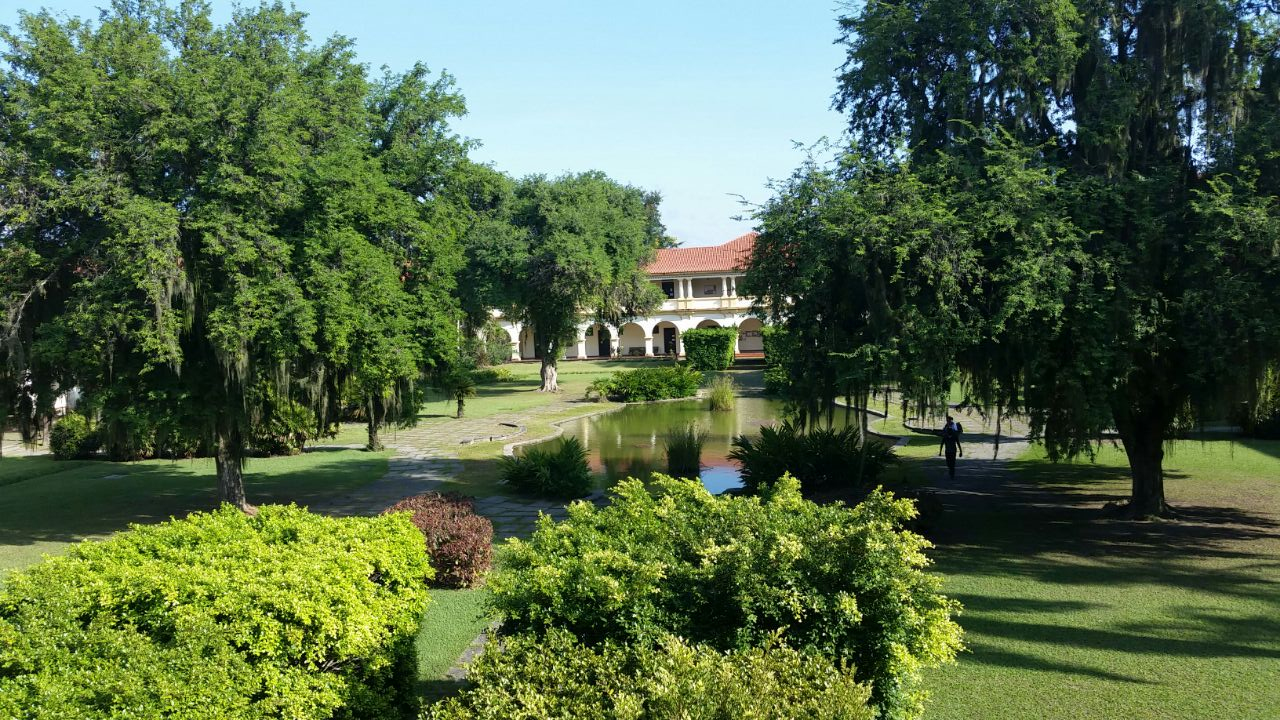
\includegraphics[scale=0.1]{RuralP1}
   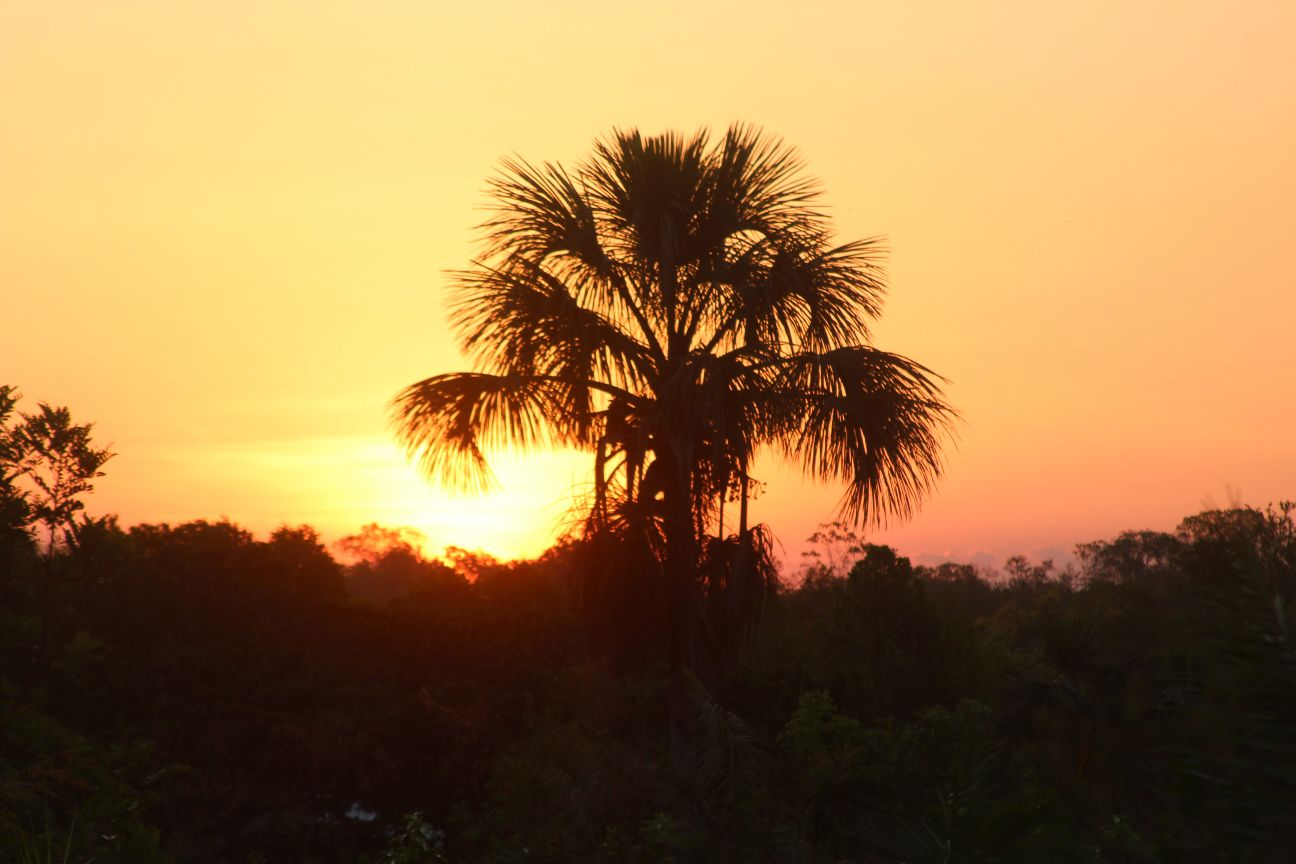
\includegraphics[scale=0.1]{Pordosol}
   \caption{Imagens lado a lado}\label{ladoalado}
\end{figure}
\end{lstlisting}
\end{tcolorbox}

\begin{figure}[H]
	\centering
	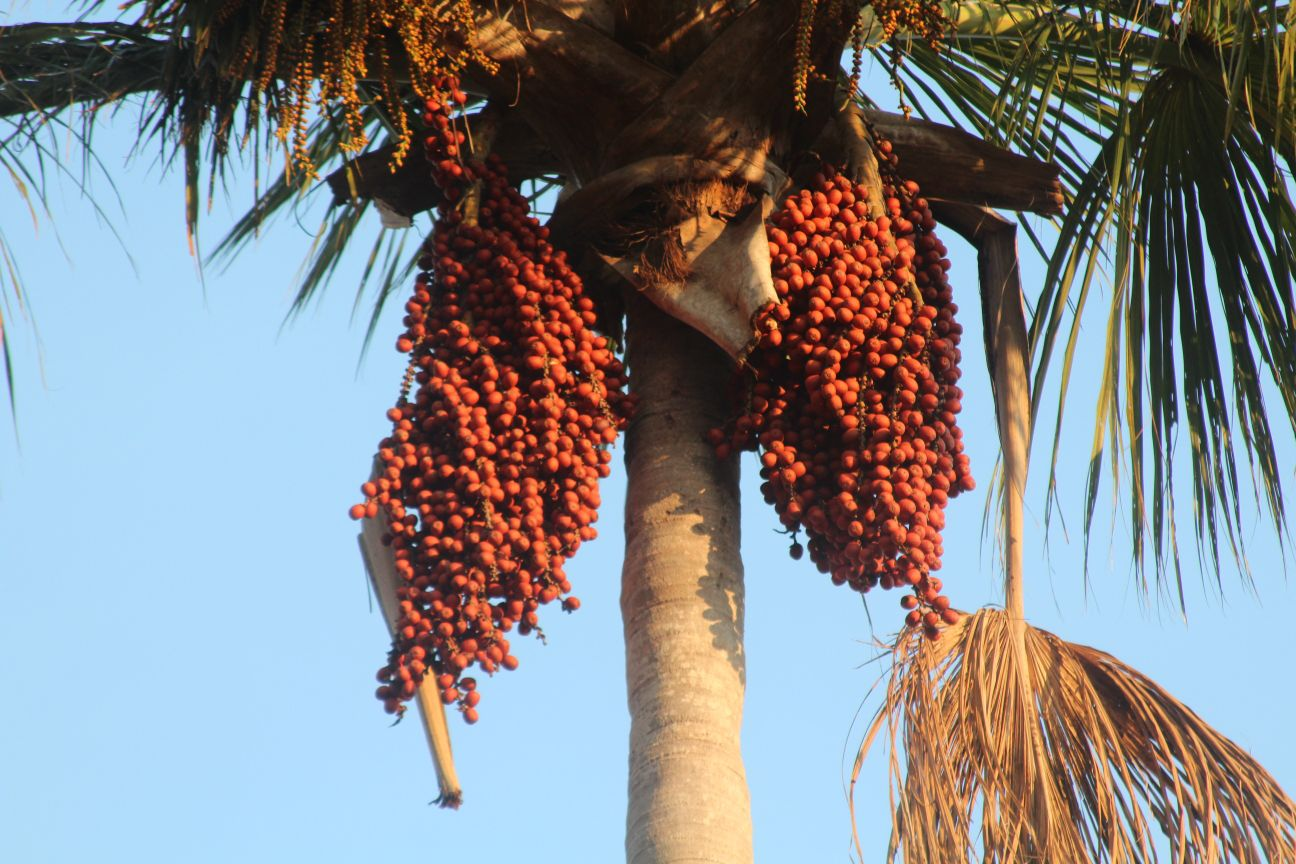
\includegraphics[scale=0.1]{Buriti}
	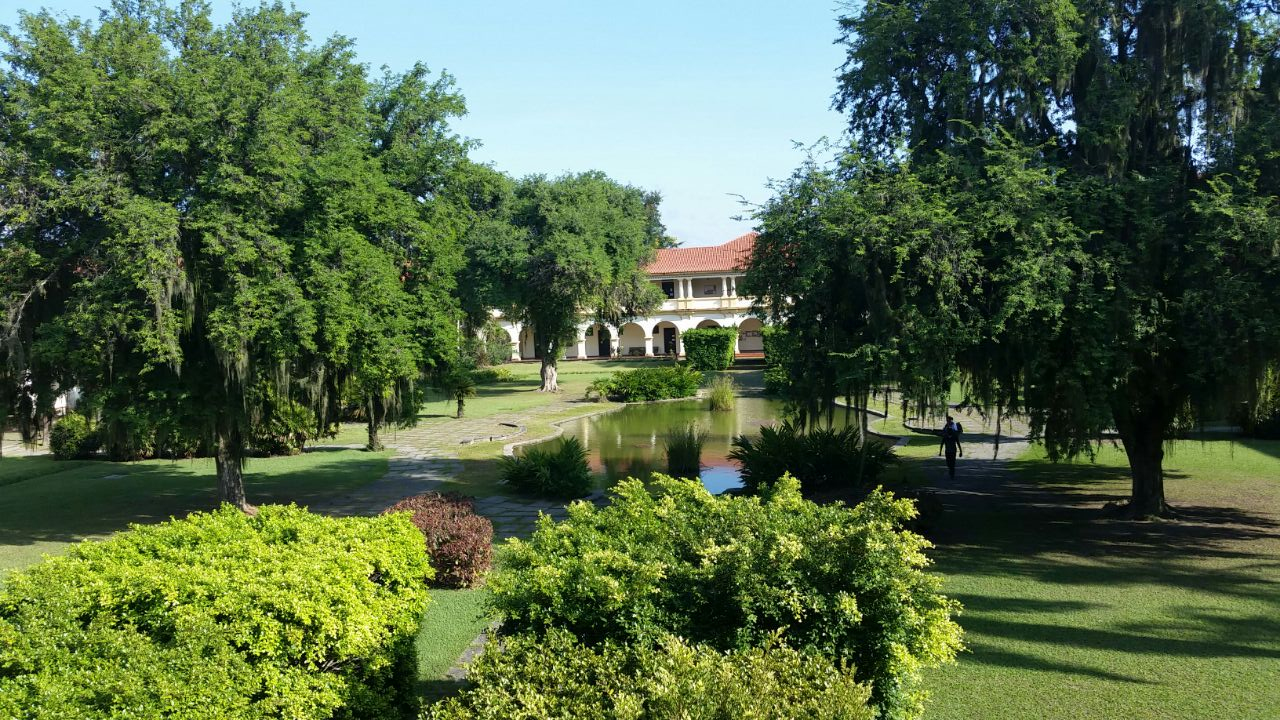
\includegraphics[scale=0.1]{RuralP1}
	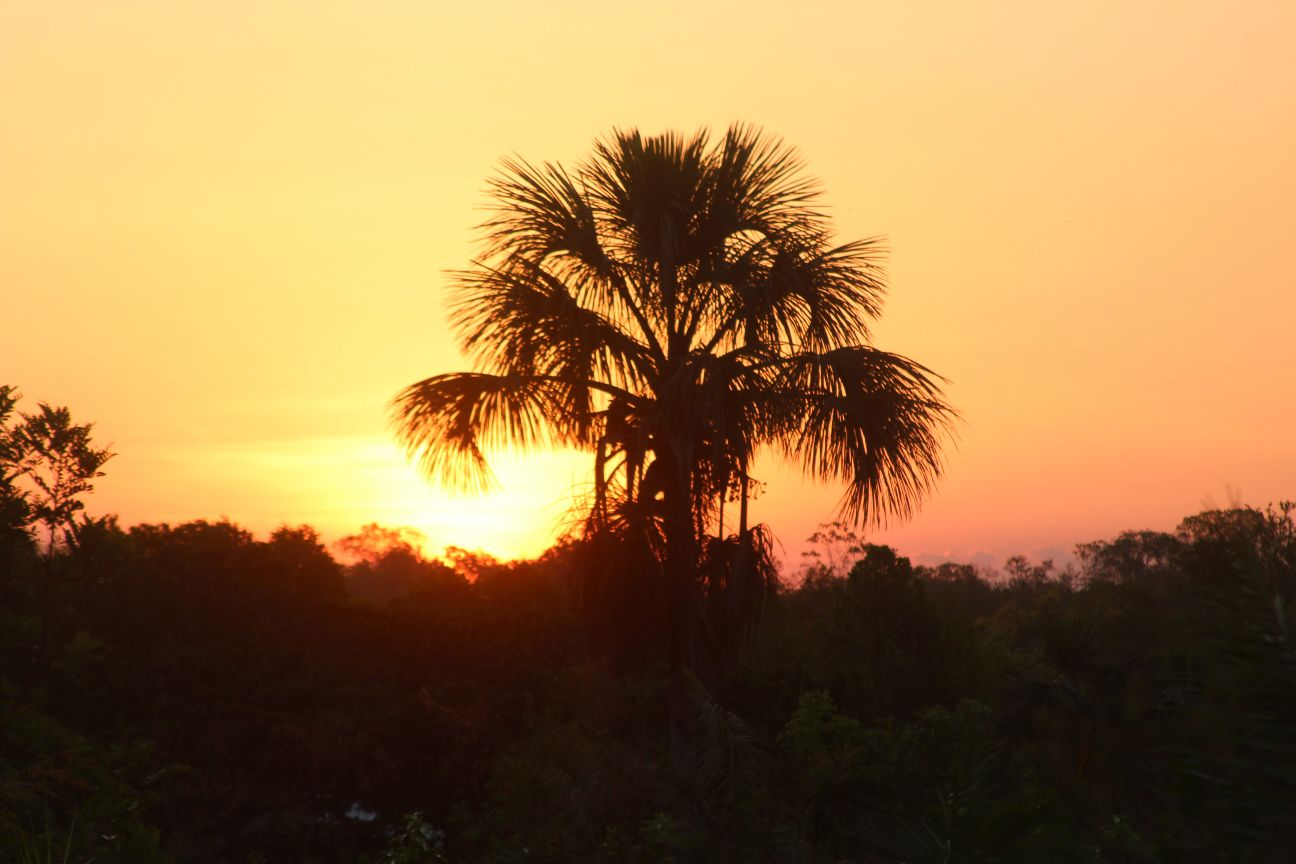
\includegraphics[scale=0.1]{Pordosol}
	\caption{Imagens lado a lado}\label{ladoalado}
\end{figure}

Para inserir uma legenda para cada figura e uma legenda geral tem-se a seguinte opção
\begin{tcolorbox}
\begin{lstlisting}
\begin{figure}[H]
   \centering
   \subcaptionbox{Fruta do buriti \label{fruta}}[0.33\linewidth]{%
		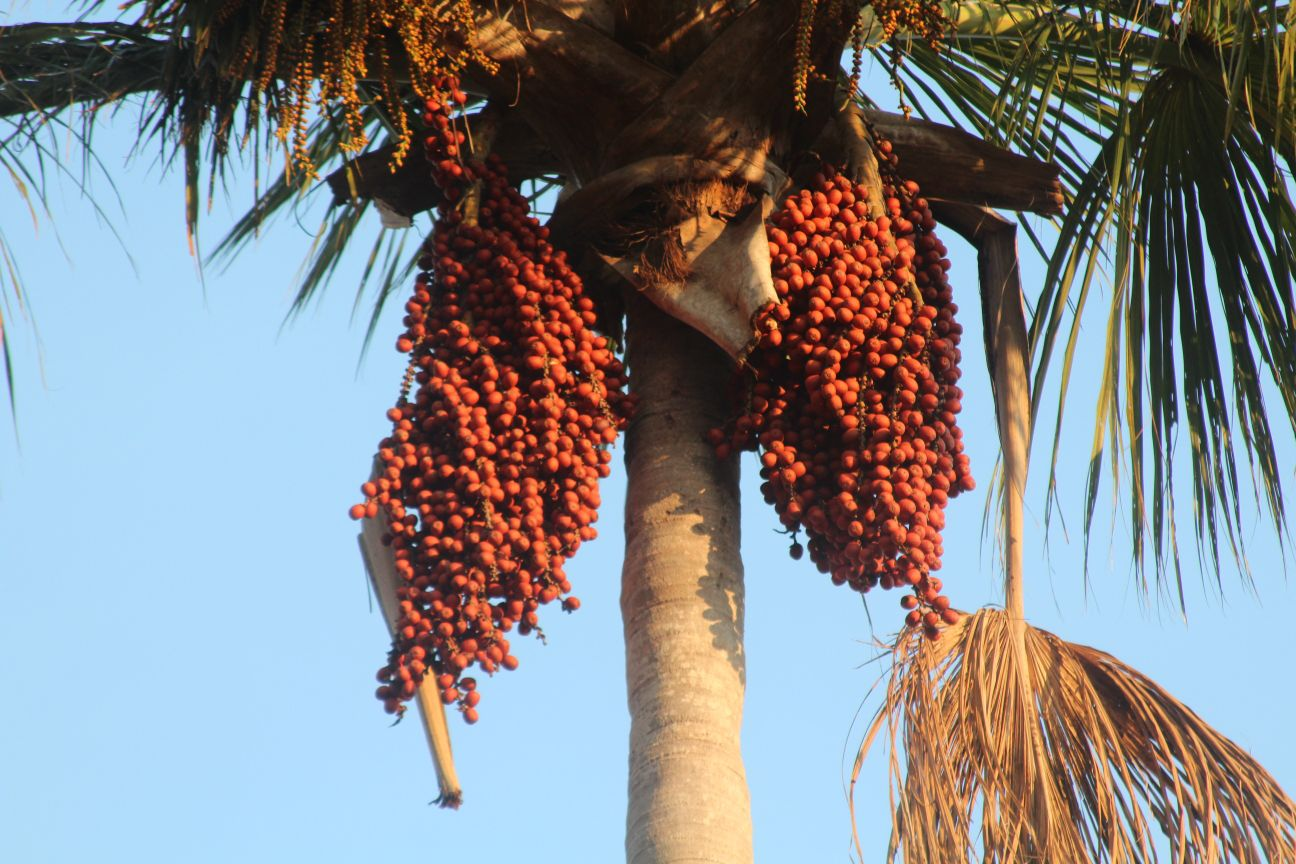
\includegraphics[scale=0.1]{Buriti}} %
   \subcaptionbox{Bonito por do sol e uma sublegenda intencionalmente
        grande\label{Pordosol}}[0.33\linewidth]{%%%
        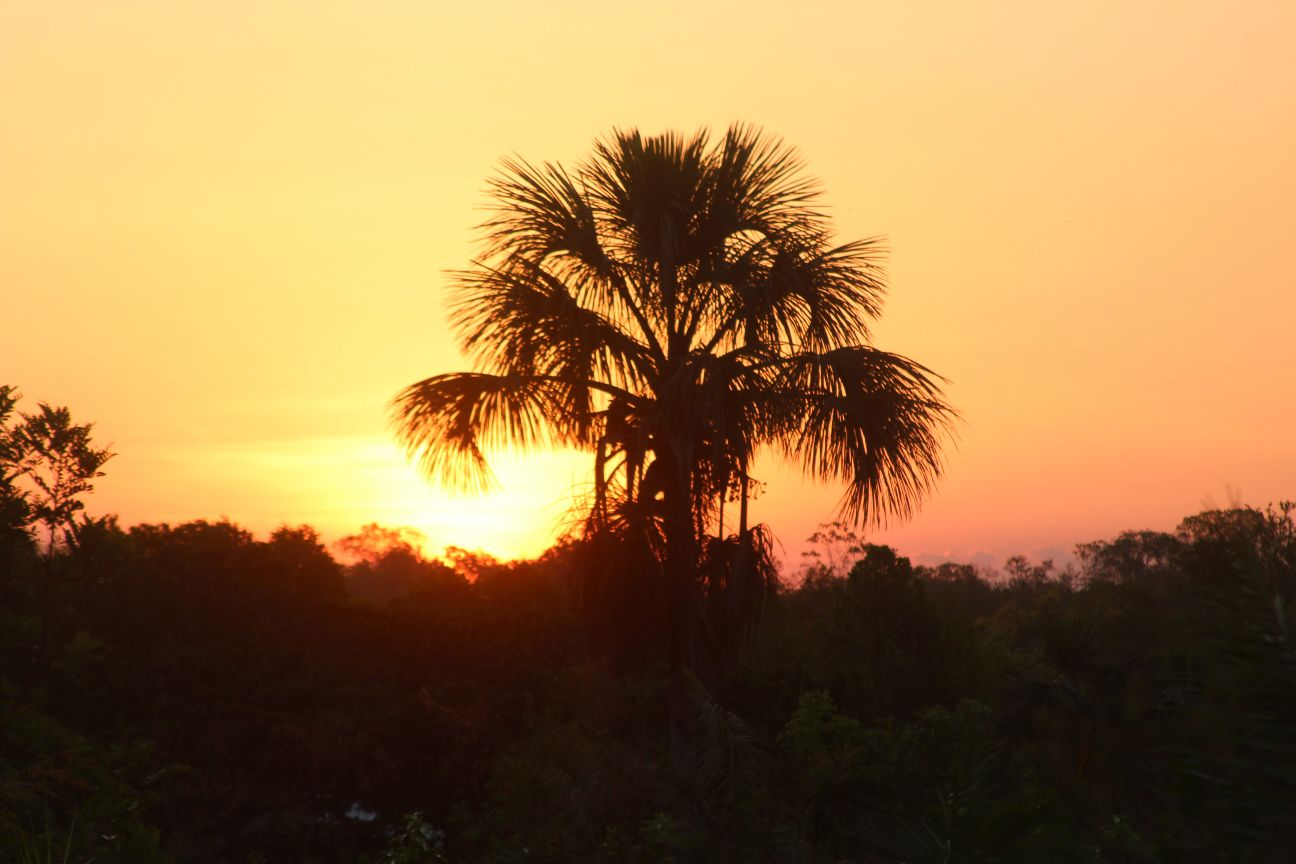
\includegraphics[scale=0.1]{Pordosol}}
   \subcaptionbox {Duas palmeiras de buriti \label{duas}}[%%%
        0.3\linewidth]{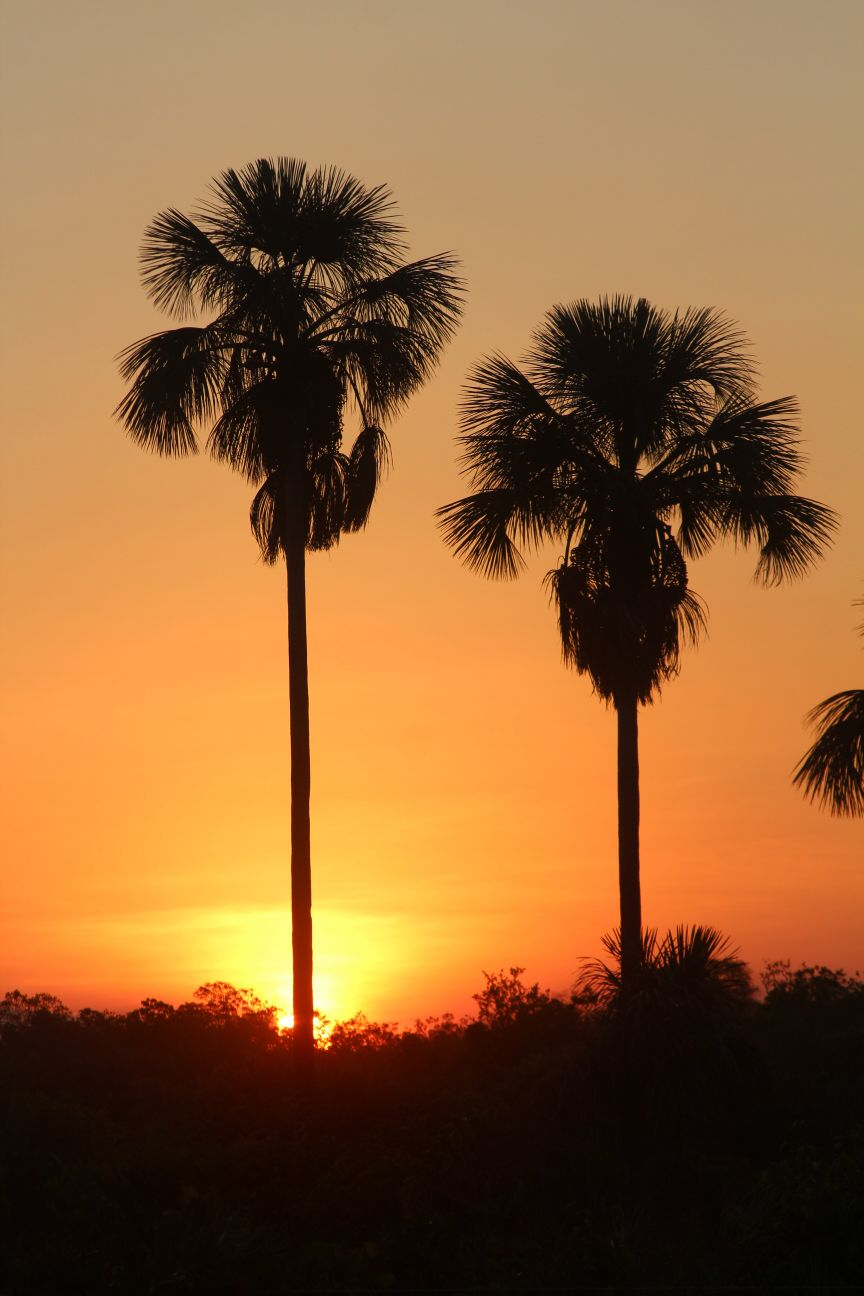
\includegraphics[scale=0.12]{Buritis}} %
   \caption{Buriti é uma palmeira de fruto saboroso}\label{buritis}
\end{figure}
\end{lstlisting}
\end{tcolorbox}
\begin{figure}[H]
	\centering
	\subcaptionbox{Fruta do buriti \label{fruta}}[0.33\linewidth]{%
		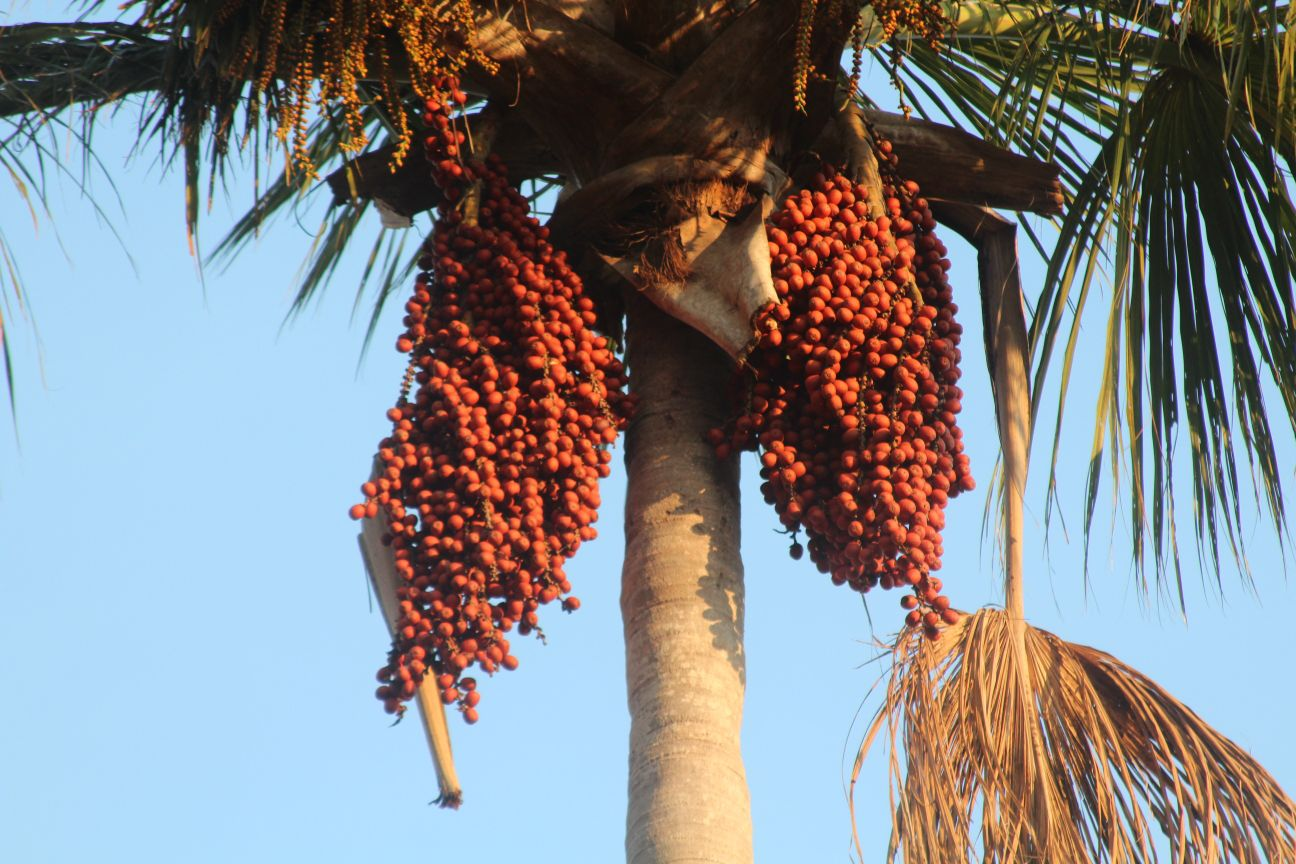
\includegraphics[scale=0.1]{Buriti}} %
	\subcaptionbox{Bonito por do sol e uma sublegenda intencionalmente grande
		\label{Pordosol}}[0.33\linewidth]{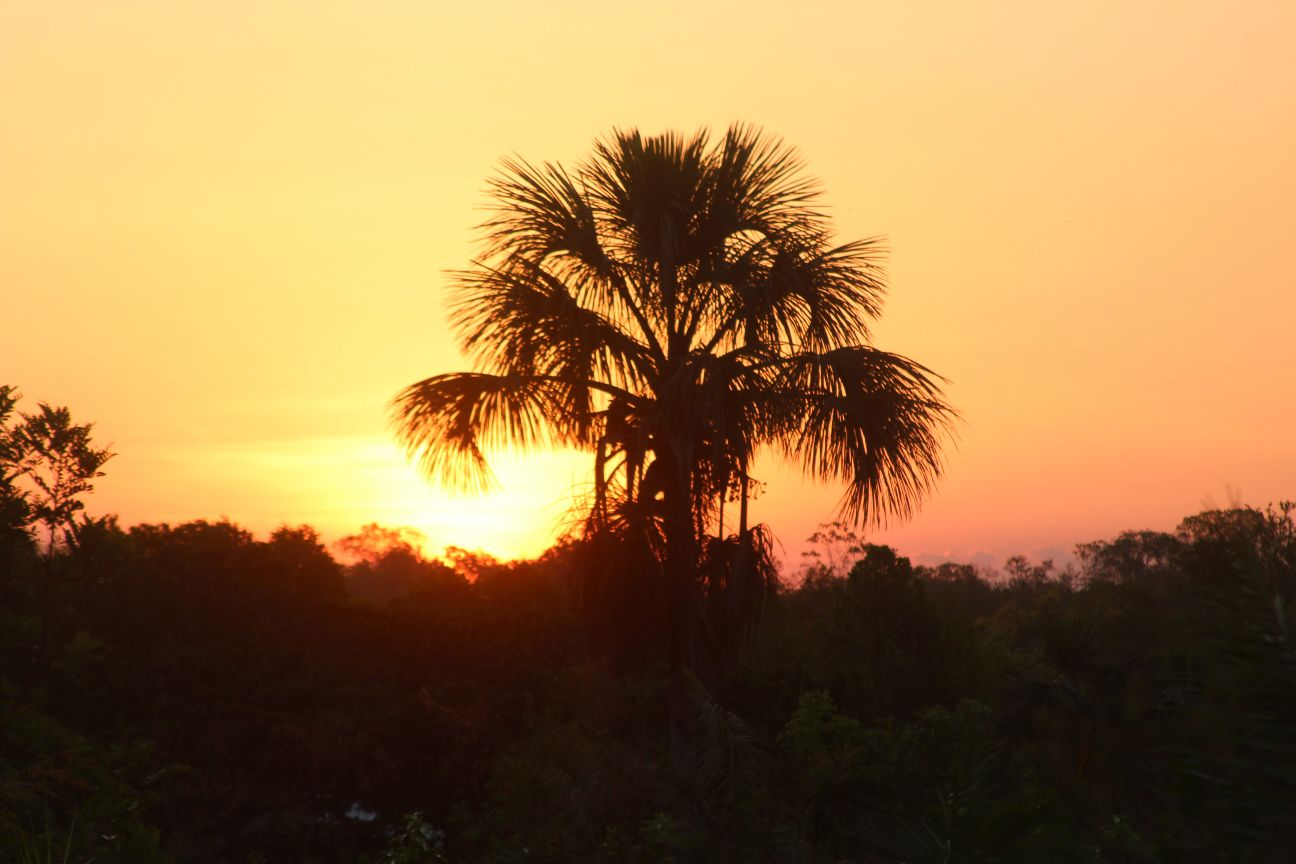
\includegraphics[scale=0.1]{Pordosol}}
	\subcaptionbox {Duas palmeiras de buriti \label{duas}}[0.3\linewidth]{%%%
		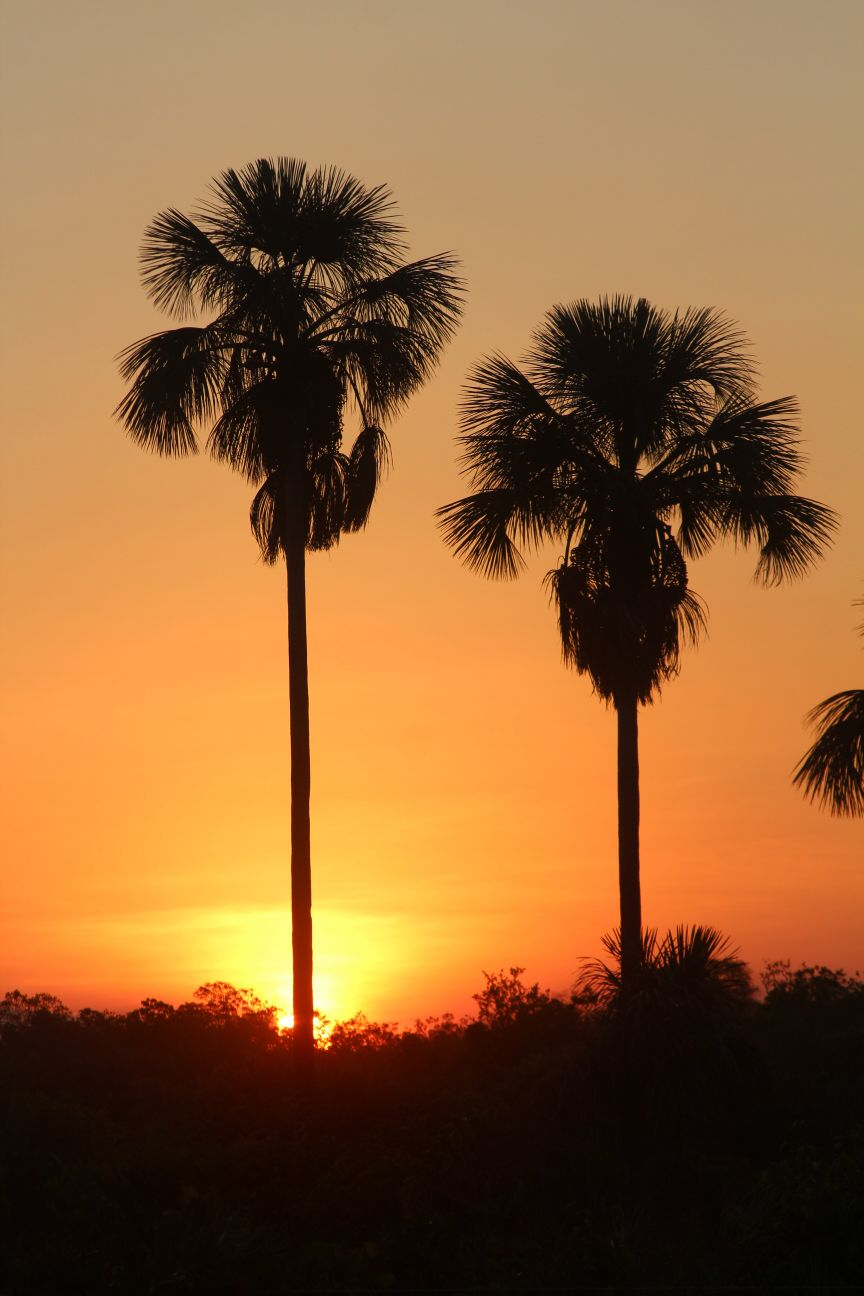
\includegraphics[scale=0.12]{Buritis}} %
	\caption{Buriti é uma palmeira de fruto saboroso}\label{buritis}
\end{figure}


\section{Inclusão de imagem com a classe estilo}

O comando para inserir imagem é o \verb|\includegraphics{imagem}|. 
Alternativamente a classe estilo definiu os comandos: \verb|\imagem| e 
\verb|\imagemlp|. Esses comandos são muito parecidos, o primeiro insere a imagem 
em tamanho natural, o segundo ajusta a largura da imagem à largura da página sem 
provocar distorções, ambos possuem três argumentos, um opcional e dois 
obrigatórios. Veja o manual.


Tanto o \verb|\imagem| quanto o \verb|\imagemlp| inserem a imagem dentro de um ambiente \texttt{table} carregado com o posicionador H, isso implica que a imagem ficará onde foi inserida de qualquer jeito.

Além de seu nome ser mais simples e fácil de manipular, esses dois comandos se encarregam de inserir todos os bons adereços que uma imagem em geral requer, tornando significativamente mais simples a manipulação de imagem.

A imagem~\ref{primeira} foi inserida com o código
\begin{tcolorbox}
\begin{lstlisting}
\begin{figure}[H]
   \centering
   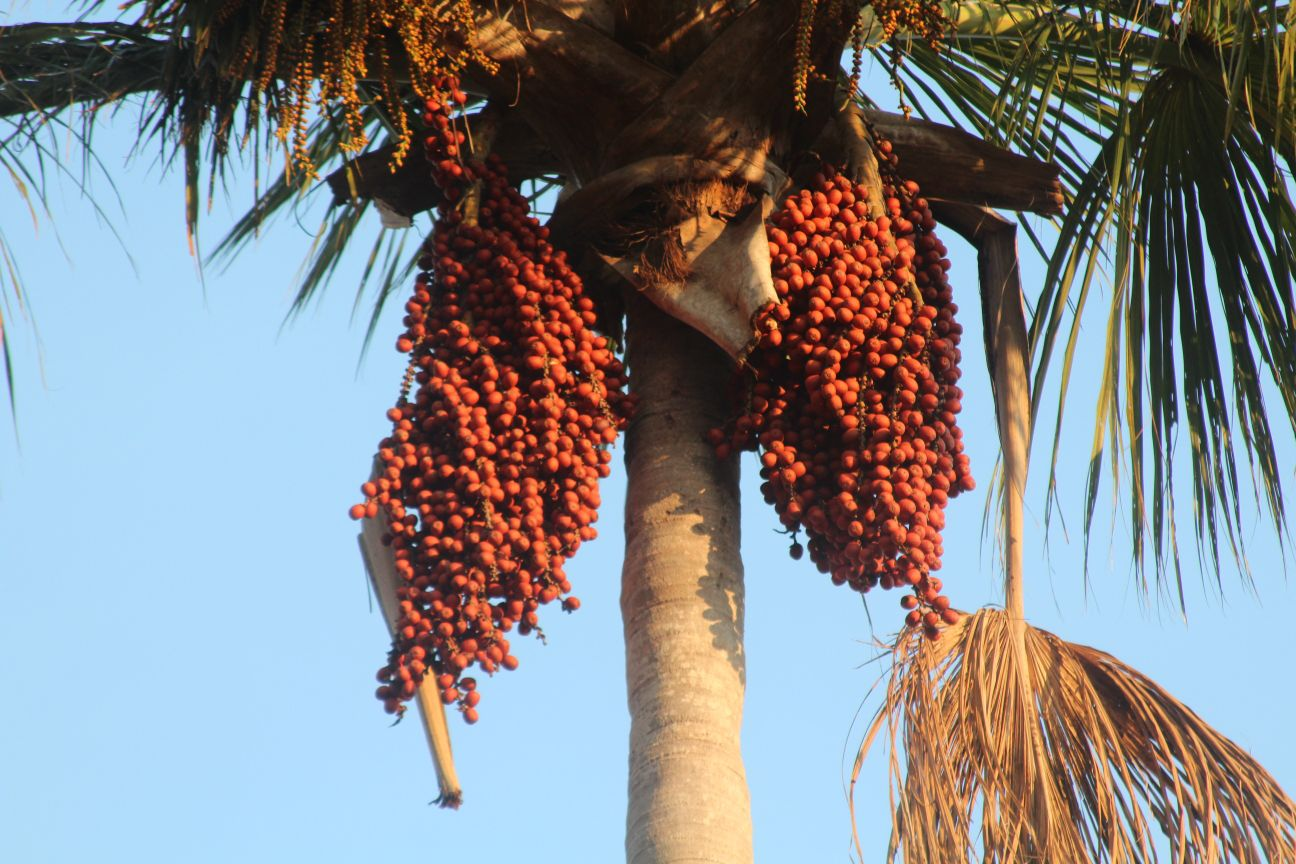
\includegraphics[scale=0.15]{Buriti}
   \caption{Imagem reduzia a $15\%$ do seu tamanho}
\end{figure}
\end{lstlisting}
\end{tcolorbox}

O mesmo resultado é obtido com o singelo fragmento
\begin{tcolorbox}
\begin{lstlisting}
\imagem[scale=0.15]{Buriti}{Imagem reduzia a $15\%$ do seu tamanho}
\end{lstlisting}
\end{tcolorbox}
\imagem[scale=0.15]{Buriti}{Imagem reduzia a $15\%$ do seu tamanho}

Da mesma forma, a imagem~\ref{op1} foi inserida com o código
\begin{tcolorbox}
\begin{lstlisting}
\begin{figure}[H]
   \resizebox{\textwidth}{!}{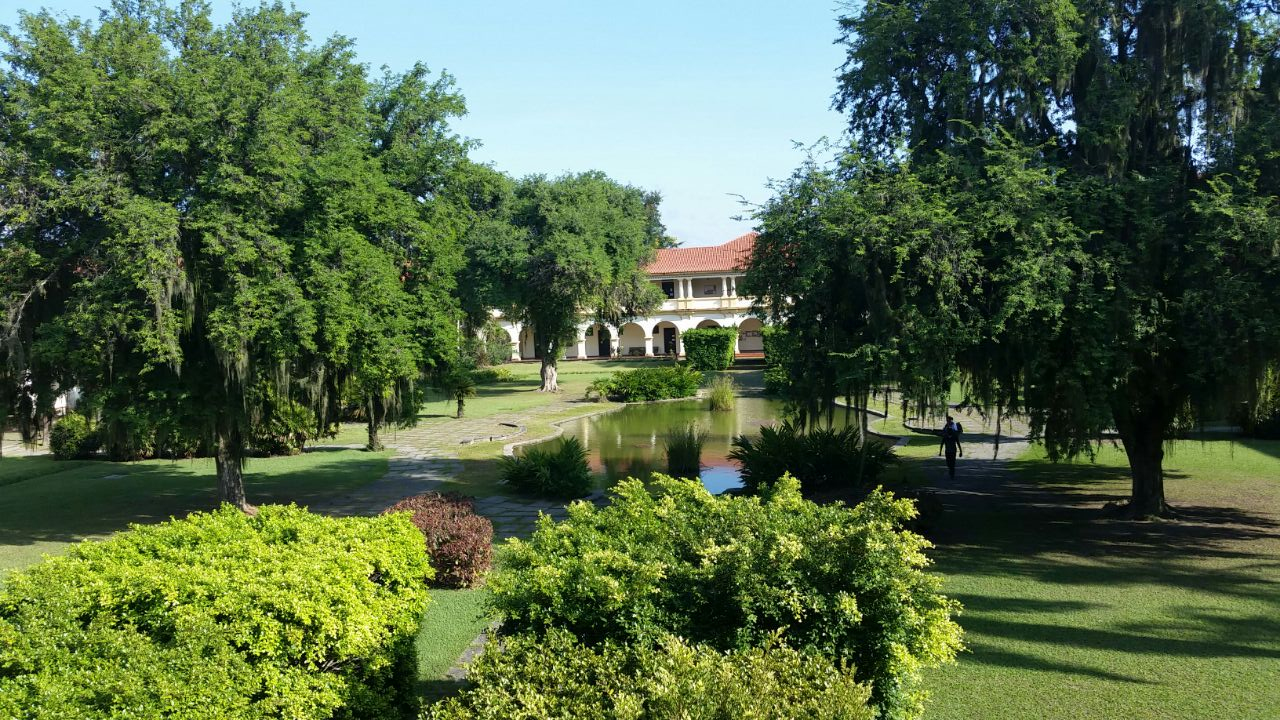
\includegraphics{RuralP1}}
   \caption{O prédio principal da UFRRJ, vulgo P1}
   \label{op1} %%% Marca para referência cruzada
\end{figure}
\end{lstlisting}
\end{tcolorbox}

O mesmo resultado é obtido com o código
\begin{tcolorbox}
\begin{lstlisting}
\imagemlp{RuralP1}{O prédio principal da UFRRJ, vulgo P1}
\end{lstlisting}
\end{tcolorbox}
\imagemlp{RuralP1}{O prédio principal da UFRRJ, vulgo P1}


\begin{tcolorbox}
\begin{lstlisting}
   Note que a imagem~\ref{RuralP1} foi ajustada para a largura da página, enquanto a imagem~\ref{Buriti}, por meio do argumento opcional $scale=0.15$, teve seu tamanho reduzido a $15\%$.
\end{lstlisting}
\tcblower
Note que a imagem~\ref{RuralP1} foi ajustada para a largura da página, enquanto a imagem~\ref{Buriti}, por meio do argumento opcional $scale=0.15$, teve seu tamanho reduzido a $15\%$.
\end{tcolorbox}

Observe como a referência cruzada foi feita utilizando o próprio nome do arquivo da imagem, sem necessidade de incluir o \verb|\label{RuralP1}| e \verb|\label{Buriti}|, essa é uma vantagem de usar os comandos da classe estilo.

\imagem{Esquema}{Imagem em pdf}